%%
%  ******************************************************************************
%  * #file    Szablon_raportu_EN_Latex.tex
%  * #author  Adrian Wójcik   adrian.wojcik(at)put.poznan.pl
%  *          
%  * #commit  Patryk Kościk   koscikpatryk(at)gmail.com
%  *          Modified the template for Projekt przejsciowy purposes          
%  *          
%  * #version 1.0
%  * #date    09-Mar-2022
%  * #brief   PROJPRZEJ
%  *
%  ******************************************************************************
%%  
\documentclass[11pt, a4paper]{article}

\usepackage{Szablon_raportu_EN_Latex}

% Wypełnijcie te dyrektywy zgodnie z waszym tematem
% \lab      -> NAZWA CZUJNIKA, np.: 'DHT22'
% \comment  -> Króciutki opis co to, np.: 'Cyfrowy budżetowy czujnik temperatury'
%
\lab{Moduł KY-040}
\comment{Czujnik obrotu, enkoder }
\author{Hubert Pietrzak}

% Absolutny zakaz dotykania tego tutaj bo jak dotkiecie to coś jebnie
\university{Politechnika Poznańska}
\faculty{Wydział Automatyki, Robotyki i Elektrotechniki}
\institute{Instytut Robotyki i Inteligencji Maszynowej}
\department{Zakład Sterowania i Elektroniki Przemysłowej}
\addbibresource{Szablon_raportu_EN_Latex.bib}
\nocite{*}


%%
%
% Początek dokumentu
%
%%
\begin{document}

%% Strona tytułowa %%
\mainpage{Enkoder}
\newpage

\section*{Opis elementu} \addcontentsline{toc}{section}{Wstęp}

Czujnik obrotu KY-040 to enkoder inkrementalny. Enkoder ma za zadanie generować impulsy, które odpowiadają ruchowi obrotowemu. Moduł może wykrywać obrót zgodnie ze wskazówkami zegara oraz przeciwnie. Czujnik zasilamy napięciem 5V jak i 3.3V. Wysyła 30 impulsów w trakcie pełnego obrotu. Enkoder inkrementalny nie generuje położenia bezwględnego. Oznacza to, że w przypadku braku zasilania wartość położenia naliczana jest od zera, to znaczy od miejsca zatrzymania się obrotu.


\vspace{0.5cm}
\begin{figure}[h]
\centering
\begin{subfigure}{.5\textwidth}
  \centering
  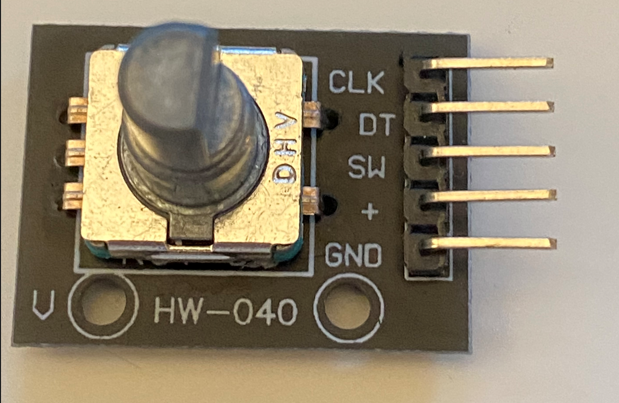
\includegraphics[width=.69\linewidth]{fig/obrazki/zdj_modułu/przód.png}
  \caption{Frontalny pogląd na enkoder inkrementalny}
  \label{fig:sub1}
\end{subfigure}%
\begin{subfigure}{.5\textwidth}
  \centering
  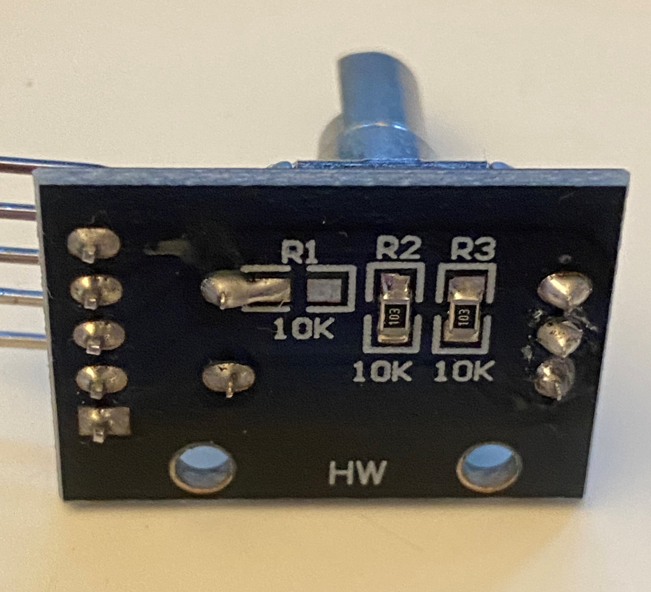
\includegraphics[width=.48\linewidth]{fig/obrazki/zdj_modułu/tyl_.png}
  \caption{Podgląd na tylną część}
  \label{fig:sub2}
\end{subfigure}
\caption{Czujnik obrotu z przodu jak i z tyłu}
\label{fig:test}
\end{figure}
\vspace{0.5cm}

%\subsection{Zasada działania}

W enkoderze inkrementalnym mamy pięć wyprowadzeń pinów. Zasilanie "$+$",GND oraz trzy wyjścia cyfrowe \textbf{CLK}, \textbf{DT} oraz \textbf{SW}, które podłączamy do wyprowadzeń mikrokontrolera. Pin \textbf{SW} służy do obsługi wbudowanego monostabilnego przycisku który po wciśnięciu wysyła pojedynczy sygnał. Monostabilny oznacza, że przycisk powraca do swojej pozycji po usunięciu siły zewnętrznej, której zadaniem najczęściej jest załączanie lub rozłączanie danego obwodu. CLK i DT służą jako dwa podstawowe kanały do identyfikacji kierunku obrotu wałka i są przesunięte w fazie o $90^{\circ}$. Mikrokontroler porównuje, który sygnał zgłasza się jako pierwszy i wykrywa kierunek obrotu enkodera, co możemy zaobserwować na poniższej grafice obrazującej to działanie.

\vspace{0.5cm}
\begin{figure}[h]
\centering
\begin{subfigure}{.5\textwidth}
  \centering
  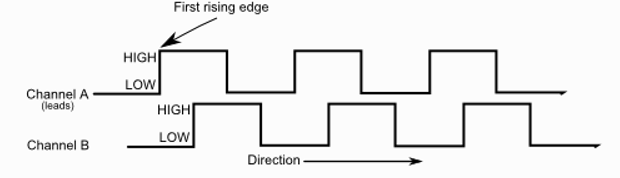
\includegraphics[width=.78\linewidth]{fig/obrazki/zasada_dzialania/opis1.png}  
  \caption{Obrót czujnika zgodnie z wskazówkami zegara}
  \label{fig:sub1}
\end{subfigure}%
\begin{subfigure}{.5\textwidth}
  \centering
  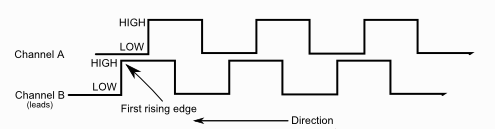
\includegraphics[width=.8\linewidth]{fig/obrazki/zasada_dzialania/opis2.png}
  \caption{Obrót czujnika przeciwnie do wskazówek zegara}
  \label{fig:sub2}
\end{subfigure}
\caption{Prezentacja wykrycia kierunku obrotu enkodera}
\label{fig:test}
\end{figure}
\vspace{0.5cm}

%\subsection{Zastosowania}
Czujniki obrotowe mogą być wykorzystywane do pomiaru przebytej drogi drogi (na przykład gdy wykorzystamy przekładnie do zamiany ruchu obrotowego w postępowy). Enkoder może też służyć jako pokrętło do zadania jakiejś konkretnej wartości (na przykład kąt), jest też wykorzystywany między innymi w automatyce przemysłowej.


\newpage

%\section{Implementacja czujnika}


% \vspace{0.5cm}

% \vspace{0.5cm}
% \begin{figure}[h!]
%     \centering
%     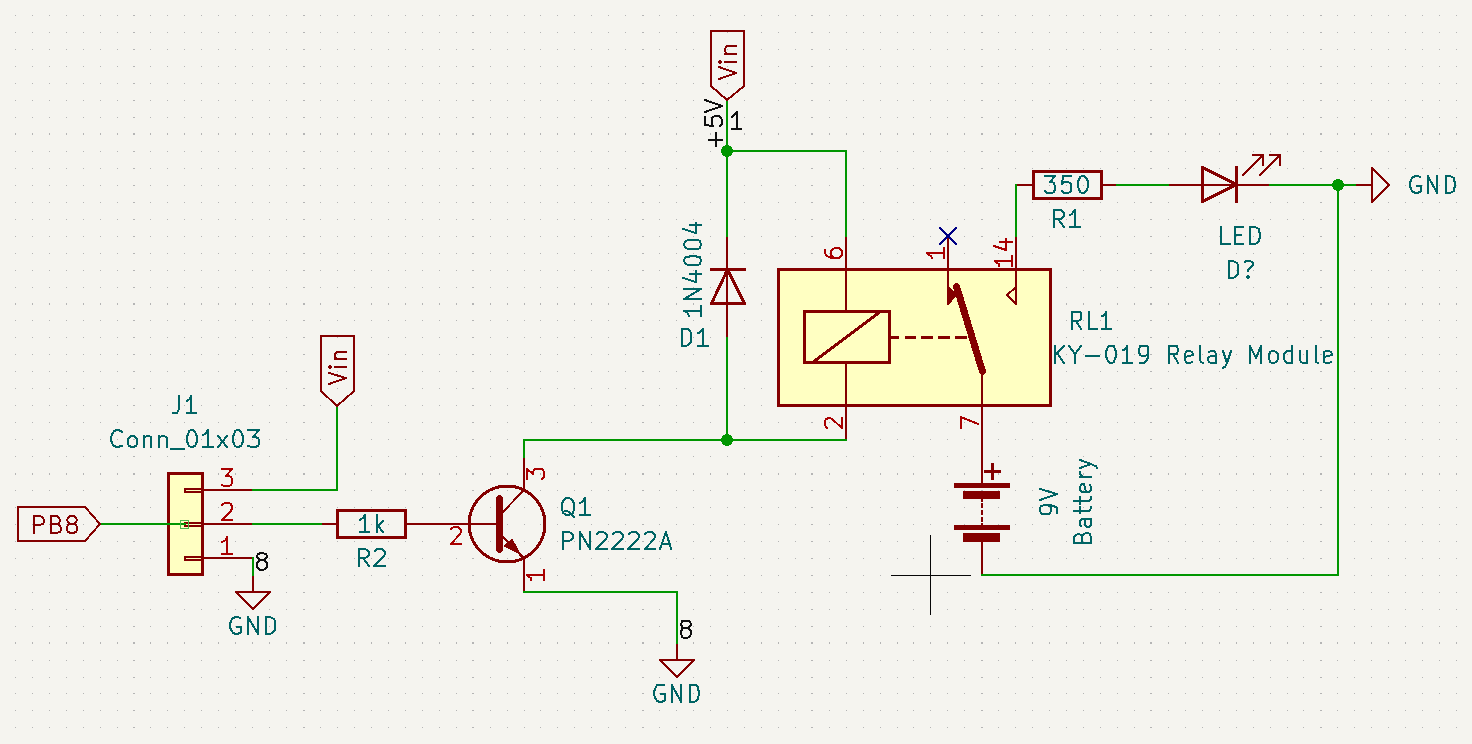
\includegraphics[scale=0.53]{fig/obrazki/polaczenie_modulu/Schematki.png}
%     \caption{Połaczenie elektryczne}
%     \label{fig:my_label}
% \end{figure}
% \vspace{0.5cm}


\newpage

%\section{Prezentacja działania układu}
\section{Użycie czujnika}

% \vspace{0.5cm}
% \begin{figure}[h!]
%     \centering
%     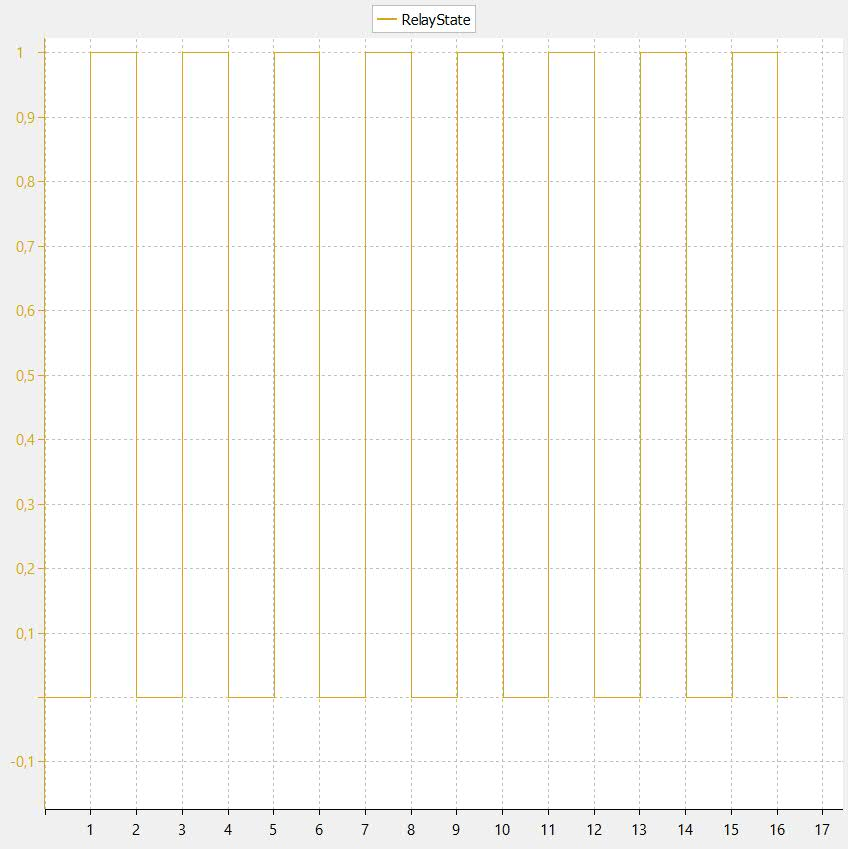
\includegraphics[width=0.6\textwidth]{fig/obrazki/działanie_ukladu/SWV.jpeg}
%     \caption{Przykładowy zrzut ekranu z SWV}
%     \label{fig:my_label}
% \end{figure}
% \vspace{0.5cm}

% W określonych chwilach czasowych (tutaj przykładowo 1 sekunda) dzięki pinowi sterującemu, przekazujemy (lub też nie) sygnał na wyjście przekaźnika, co obserwujemy zmieniającym się stanem zmiennej \textbf{RelayState}

\vspace{0.5cm}
\begin{figure}[h!]
    \centering
    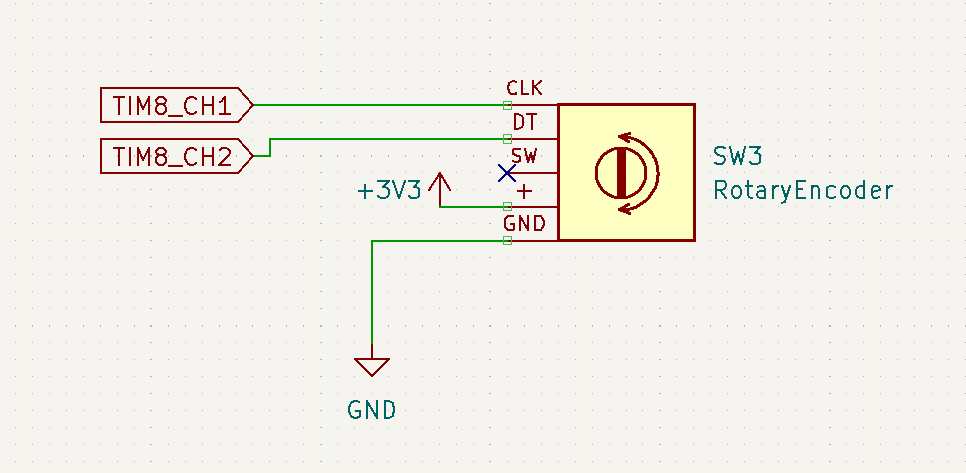
\includegraphics[scale=0.70]{fig/obrazki/polaczenie_modulu/SCHEMAT.png}
    \caption{Schemat podłączeń modułu}
    \label{fig:my_label}
\end{figure}
\vspace{0.5cm}

\vspace{0.5cm}
\begin{figure}[h!]
    \centering
    \includegraphics[scale=0.70]{Podłaczenie-removebg-preview.png}
    \caption{Fizyczne podłączenie}
    \label{fig:my_label}
\end{figure}
\vspace{0.5cm}



\vspace{0.5cm}
\begin{figure}[h!]
    \centering
    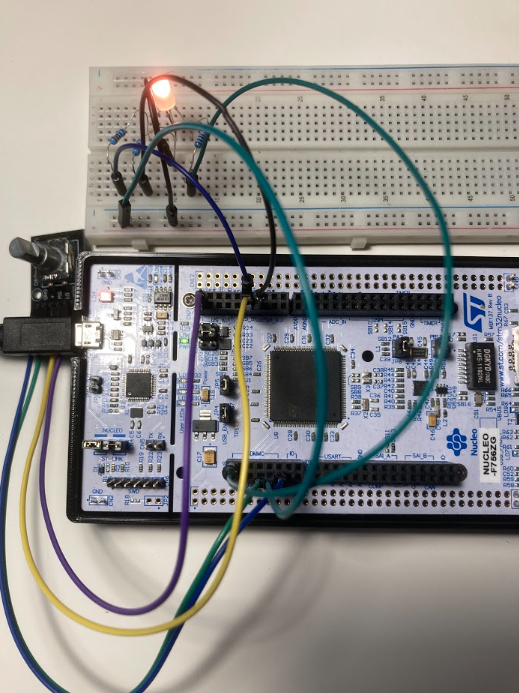
\includegraphics[scale=0.8]{fig/obrazki/działanie_ukladu/PELNEZDJECIE.png}
    \caption{Rzeczywista realizacja układu z dodatkowym sterowaniem barwą diody RGB}
    \label{fig:my_label}
\end{figure}
\vspace{0.5cm}

% Na załączonej fotografii obserwujemy prawidłowe podłączenie enkodera do odpowiednich pinów zgodnie ze schematem oraz dołączonym sterowaniem kolorem diody RGB z dodatkowymi trzema kanałami podłączonymi do mikrokontrolera w celu sterowania barwą dla zadanego kątu obrotu modułu KY-040. Jest to jedno z najprostszych zastosowań wykorzystania czujnika obrotu.


% \vspace{0.5cm}
% \begin{figure}[h!]
%     \centering
%     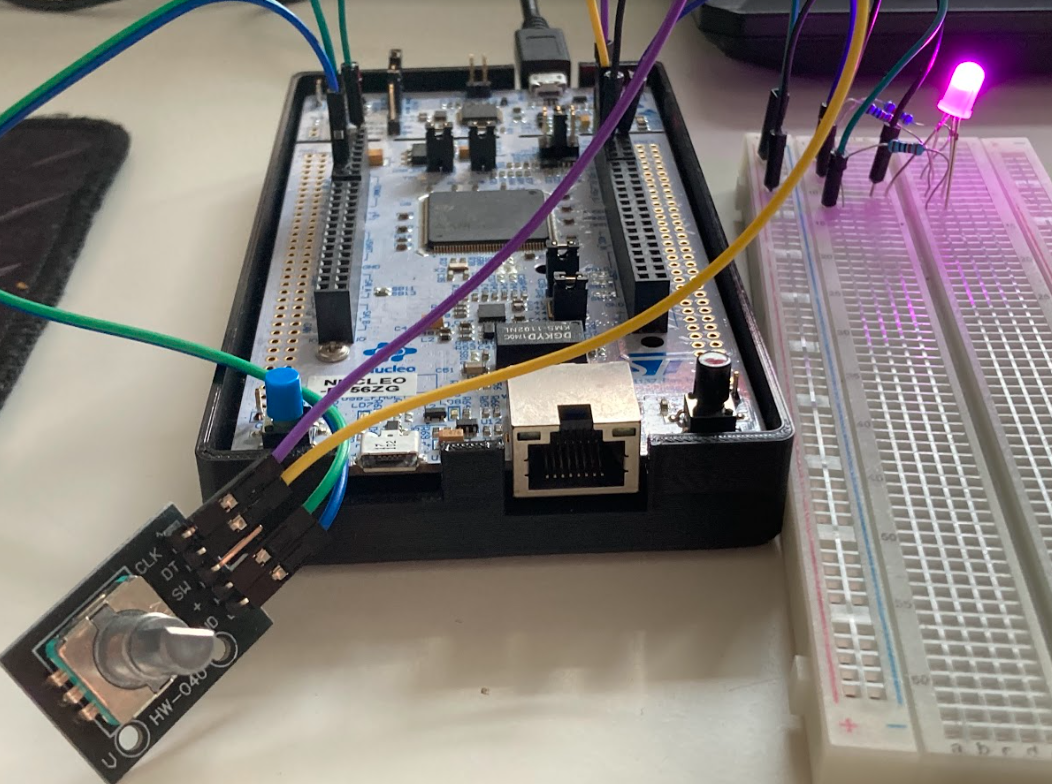
\includegraphics[scale=0.5]{fig/obrazki/działanie_ukladu/pozycja2.png}
%     \caption{Położenie enkodera i odpowiadająca mu barwa}
%     \label{fig:my_label}
% \end{figure}
% \vspace{0.5cm}


% \vspace{0.5cm}
% \begin{figure}[h!]
%     \centering
%     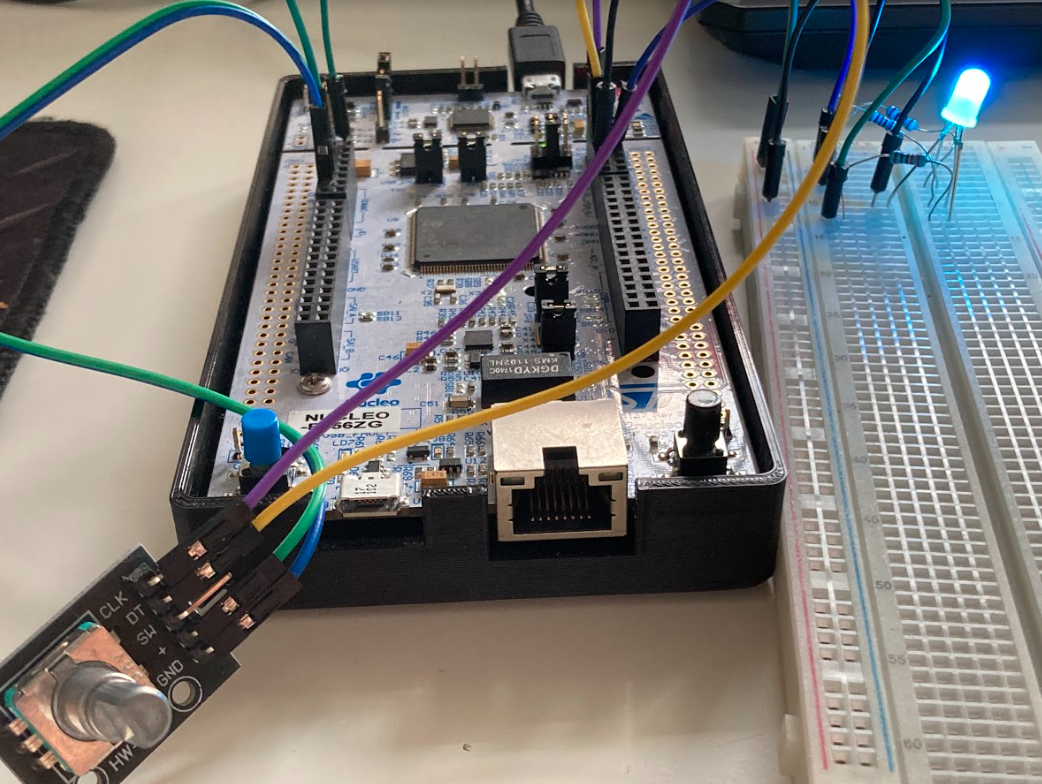
\includegraphics[scale=0.52]{fig/obrazki/działanie_ukladu/pozycja1.png}
%     \caption{Zmiana położenia czujnika obrotu skutkująca innym kolorem diody}
%     \label{fig:my_label}
% \end{figure}
% \vspace{0.5cm}

% % \vspace{0.5cm}
% % \begin{figure}[h!]
% %     \centering
% %     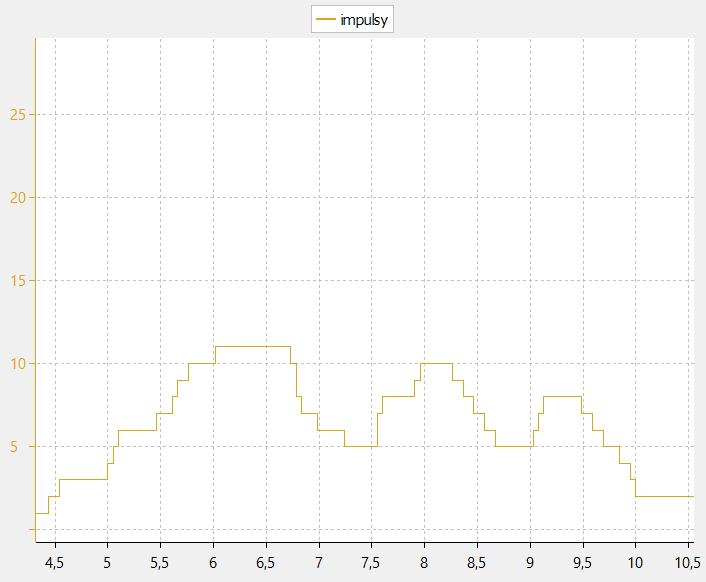
\includegraphics[scale=0.4]{fig/obrazki/działanie_ukladu/IMPULSY_PRZEBIEG.png}
% %     \caption{Przebieg zmiany impulsów od czasu (obracanie enkoderem)}
% %     \label{fig:my_label}
% % \end{figure}
% % \vspace{0.5cm}


\newpage

\section*{Podsumowanie} \addcontentsline{toc}{section}{Podsumowanie}
Enkoder inkrementalny jest sensorem, który kontroluje kąt obrotu o jaką nastąpiło przesunięcie względem początkowego położenia i działa 'krokowo' (cały obrót jest podzielony na impulsy), zmianę położenia kątowego wykrywają te impulsy, których dla tego konkretnego czujnika jest 30 oraz zawiera wbudowany przycisk. 



\printbibliography[heading=bibintoc]

\end{document}